\chapter{Distribuzione e Packaging} \label{chap:distribuzione_packaging}

    Il software Indico, come già accennato, è un software open source, principalmente sviluppato al \ac{CERN}. Il codice di Indico viene aggiornato regolarmente, producendo ogni volta nuove versioni di Indico. Data la vastità della community di Indico, ogni volta che viene rilasciata una nuova versione il team di Indico al \ac{CERN} deve occuparsi di creare una distribuzione di Indico relativa a quella versione e quindi di distribuirla attraverso i principali canali di comunicazione. Non solo, un amministratore di una qualche istanza Indico, o magari uno sviluppatore esterno al gruppo Indico al \ac{CERN}, potrebbe sentire il bisogno di creare una distribuzione di una specifica versione di Indico per testarla o per caricarla dove più desidera. Inoltre uno sviluppatore potrebbe avere bisogno di creare diverse distribuzioni per diverse versioni di Python o anche distinguere tra distribuzione del codice sorgente e distribuzione binaria precompilata, pronta ad essere eseguita.
    
    Creare una nuova distribuzione ogni volta, personalizzandola alle proprie esigenze, e distribuirla su uno o più canali, risulta essere un processo tedioso e ripetitivo, specialmente se, per motivi di testing, si è costretti a generare molte distribuzioni in rapida successione.
    
    Con questa seconda fase del Progetto KT per Indico si è cercato proprio di risolvere questo problema, cercando di automatizzare e parametrizzare il processo di generazione e diffusione di una distribuzione Indico.
    
    L'obiettivo di questo progetto era quindi quello di scrivere uno script che automatizzasse:
    
    \begin{itemize}
        \item la creazione di distribuzioni di diverse versioni di Indico,
        \begin{itemize}
            \item sia del codice sorgente (tarball),
            \item che precompilata (Python egg);
        \end{itemize}
        \item la creazione di distribuzioni binarie per diverse versioni di Python;
        \item l'upload della distribuzione
        \begin{itemize}
            \item su un server
            \item e su GitHub.
        \end{itemize}
    \end{itemize}
    
    Con \textit{tarball} si indica comunemente la distribuzione di un pacchetto o libreria i cui file sono archiviati tramite il comando \bash{tar}, il quale genera un file in formato \bash{.tar}. Spesso, come in questo caso, i file \bash{.tar} vengono anche compressi utilizzando il comando \bash{gzip}, producendo un file in formato \bash{.tar.gz}. Solitamente le tarball vengono utilizzate per distribuire codice sorgente di programmi open source, come in questo caso. I \textit{Python egg} rappresentano invece distribuzioni di programmi Python precompilati. I Python egg sono molto utili quando non interessa il codice sorgente, in quanto per installarli basta eseguire il comando \bash{easy_install} messo a disposizione da Python stesso. Per maggiori informazioni su tarball e Python egg si vedano \cite{scholz:egg} e \cite{wiki:tar}.
    
    Lo script scritto per automatizzare la creazione di una distribuzione e l'upload è uno script Fabric (si veda la Sezione \ref{sec:p;strumenti_linguaggi}), denominato \bash{fabfile.py}, che è stato includo nel codice sorgente del progetto principale di Indico\footnote{\url{https://github.com/indico/indico}.}. Questo script era già presente prima di questo progetto ed era utilizzato per generare distribuzioni di codice sorgente e binario e per installare le dipendenze esterne necessarie a Indico. Si sono quindi aggiunte allo script le funzioni per generare distribuzioni per diverse versioni di Indico e di Python e per caricarle su un server e su un repository GitHub.\footnote{Per vedere in dettaglio le aggiunte apportate allo script da questo progetto di veda il seguente commit su GitHub: \url{https://github.com/indico/indico/commit/75ea63df8d19402d8ab47b22d77d1f7b4bf1fc79}.}
    
    La task principale di questo script Fabric si chiama \python{package_release} e la sua esecuzione si divide in due fasi: nella prima si genera la distribuzione secondo i parametri richiesti, mentre nella seconda si effettua l'upload della distribuzione generata su un server specificato e/o su un repository GitHub. Vediamo, nelle Sezioni seguenti, come funzionano queste due fasi.
    
    \section{Generazione di una distribuzione} \label{sec:dp;generazione_distribuzione}
    
        Durante la prima fase dello script di packaging, viene effettuata la generazione della distribuzione. Ad ogni esecuzione lo script permette di specificare la versione di Indico rispetto alla quale vogliamo creare la distribuzione ed una o più versioni di Python rispetto alle quali vogliamo creare le distribuzioni binarie. Prima di questo progetto, lo script era già in grado di generare tarball e Python egg, ma era limitato a farlo per la versione corrente di Indico e la versione di default di Python.
        
        Lo script, innanzitutto, si preoccupa di selezionare i file sorgenti relativi alla versione Indico selezionata. Per far questo effettua un \bash{git clone}, nel caso in cui il repository non sia presente in locale, e quindi effettua un \bash{git checkout} in modo da cambiare branch e posizionarsi nella versione desiderata. Il sistema di nomenclatura dei branch in Indico segue la convenzione che ad ogni branch corrisponde una versione ed il nome del branch è formato da una ``v'' seguita dal numero della versione (eventualmente con punti per distinguere tra versioni principali e versioni minori). Il frammento di codice relativo a questa parte è il seguente:
        
        \begin{center}
            \begin{lstlisting}[language=python, gobble=14]
                with lcd(build_dir):
                    if os.path.exists(os.path.join(build_dir, 'indico')):
                        print yellow("Repository seems to already exist.")
                        with lcd('indico'):
                            local('git fetch {0}'.format(upstream))
                            local('git reset --hard FETCH_HEAD')
                            if not no_clean:
                                local('git clean -df')
                    else:
                        local('git clone {0}'.format(upstream))
                    with lcd('indico'):
                        print green("Checking out branch \'{0}\'".format(indico_version))
                        local('git checkout {0}'.format(indico_version))
                        local('fab _package_release:{},{},{}'.format(
                            os.path.join(build_dir, 'indico'), ':'.join(py_versions), str(system_node).lower()))
            \end{lstlisting}
            \captionsetup{textformat=empty,labelformat=empty} \vspace{-2em}
            \captionof{lstlisting}[Selezione della versione di Indico per la distribuzione]{Selezione del branch corretto di Indico per la generazione di distribuzioni.}
        \end{center}
        
        Si vede che una volta effettuato il checkout del branch corretto (o \bash{master} se non viene indicato niente) lo script invoca la funzione privata \python{_package_release}, che si occupa di generare la distribuzione dei sorgenti (tarball) e la/e distribuzione/i binaria/e per ogni versione Python selezionata (sotto forma di Python egg). Le funzioni per la generazione della tarball e del Python egg erano già presenti nello script e sono state riutilizzate, aggiungendo soltanto la facoltà di generare Python egg per diverse versioni di Python.
        
        Per generare la distribuzione dei sorgenti, lo script installa e configura le dipendenze esterne di Indico e quindi procede con l'invocazione del comando \python{sdist} del modulo \python{setuptools} \cite{python:sdist}, che si occupa di generare una distribuzione dei sorgenti (il formato di default è \bash{.tar.gz}, ovvero una tarball).
        
        La generazione delle distribuzioni binarie è molto simile, con l'unica differenza che viene generata una distribuzione per ogni versione Python selezionata. In particolare, lo script utilizzerà di volta in volta un compilatore Python differente, a seconda della versione scelta, e, per ognuno di essi, invocherà il comando \python{bdist_egg}, del modulo \python{setuptools} \cite{python:bdist}, che genera una nuova distribuzione binaria sotto forma di Python egg. Per utilizzare compilatori Python differenti a seconda della versione desiderata, all'inizio dello script vengono creati tanti ambienti Python virtuali, tramite la libreria \bash{pyenv}\footnote{\url{https://github.com/yyuu/pyenv}.}, quante sono le versioni Python richieste: in ognuno di questi ambienti verrà installata una diversa versione di Python e, al momento della generazione del Python egg, non verrà semplicemente chiamato il compilatore Python globale (come veniva fatto nello script vecchio) ma si invocherà il compilatore specifico alla versione passata come argomento.
    
    \section{Upload della distribuzione} \label{sec:dp;upload_distribuzione}
    
        Una volta generate le distribuzioni desiderate, l'utente può scegliere se caricarle su GitHub, su un server oppure su entrambi. Tutte le impostazioni relative a questa fase possono essere impostate tramite il file di configurazione dello script, chiamato \bash{fabfile.conf}.
        
        \subsection{Upload su GitHub} \label{subsec:dp;ud;upload_github}
        
            GitHub rappresenta il principale mezzo di distribuzione di Indico ed è uno strumento molto potente in quanto fornisce agli sviluppatori molti strumenti di distribuzione. In GitHub si possono infatti creare delle \textit{release}, ovvero una distribuzione del software relativa ad una versione particolare. Per ogni release, inoltre, gli sviluppatori possono caricare allegare alcuni file, detti \textit{asset}, caricandoli su GitHub, in modo che gli utenti possano usufruirne. L'obiettivo della fase di upload a GitHub prevede infatti di caricare le distribuzioni generate nella fase precedente come asset della release corrispondente alla versione di Python generata.
            
            I parametri relativi a questa fase all'interno del file \bash{fabfile.conf} hanno la seguente struttura:
            
            \begin{center}
                \begin{lstlisting}[language=python, gobble=18]
                    github = {
                        'user': 'your-username',
                        'org': 'indico',
                        'repo': 'indico',
                        'auth_token': 'your-access-token',
                    
                        # What do to in case release exists
                        # True: overwrite, False: do not overwrite, None: ask
                        'overwrite': None
                    }
                    github['upstream'] = "https://github.com/{0}/{1}.git".format(github['org'], github['repo'])
                \end{lstlisting}
                \captionsetup{textformat=empty,labelformat=empty} \vspace{-2em}
                \captionof{lstlisting}[Configurazione per l'upload a GitHub (esempio)]{Esempio di parametri di configurazione per l'upload a GitHub.}
            \end{center}
            
            La fase di upload su repository GitHub prevede innanzitutto che l'utente specifichi un username e password validi per poter accedere al repository richiesto. Alternativamente alla password, l'utente può anche specificare un token OAuth valido.
            
            Una volta assicuratosi che le credenziali sono valide, lo script effettua delle richieste \ac{HTML}, tramite il pacchetto \python{requests}, per controllare se la release corrispondente alla versione Indico selezionata è già presente o meno sul repository. Nel caso in cui sia già presente, e l'utente abbia settato a \python{True} il parametro \python{overwrite}, allora si procede a sovrascrivere gli asset della release già esistente con le nuove distribuzioni generate. In caso contrario, si crea una nuova release e si caricano tutte le distribuzioni direttamente. Per fare l'upload di ogni singolo file generato si deve inviare una richiesta, contenente il file come dati, alla seguente \ac{API} messa a disposizione da GitHub:
            
            \begin{center}
                \begin{lstlisting}[language=python, gobble=18]
                    https://uploads.github.com/repos/{0}/{1}/releases/{2}/assets
                \end{lstlisting}
                \captionsetup{textformat=empty,labelformat=empty} \vspace{-2em}
                \captionof{lstlisting}[API per l'upload a GitHub]{API per l'upload di asset in una release su un repository di GitHub.}
            \end{center}
            
            Per una documentazione più dettagliata delle \ac{API} di GitHub si veda \cite{github:api}.
            
            A titolo d'esempio si può vedere la release 1.2 di Indico, raggiungibile all'indirizzo \url{https://github.com/indico/indico/releases/tag/v1.2.0}, nella quale sono state caricate automaticamente una distribuzione del codice sorgente (``Source code (tar.gz)'') e due distribuzioni binarie, relative a Python 2.6 e 2.7 (``indico-1.2-py2.6.egg'' ``e indico-1.2-py2.7.egg''), utilizzando lo script appena descritto. Il riepilogo degli asset disponibili per la versione 1.2 viene visualizzato su GitHub come in Figura \ref{fig:1_2_asset}.
            
        	\begin{figure}[h!]
        		\begin{center}
        			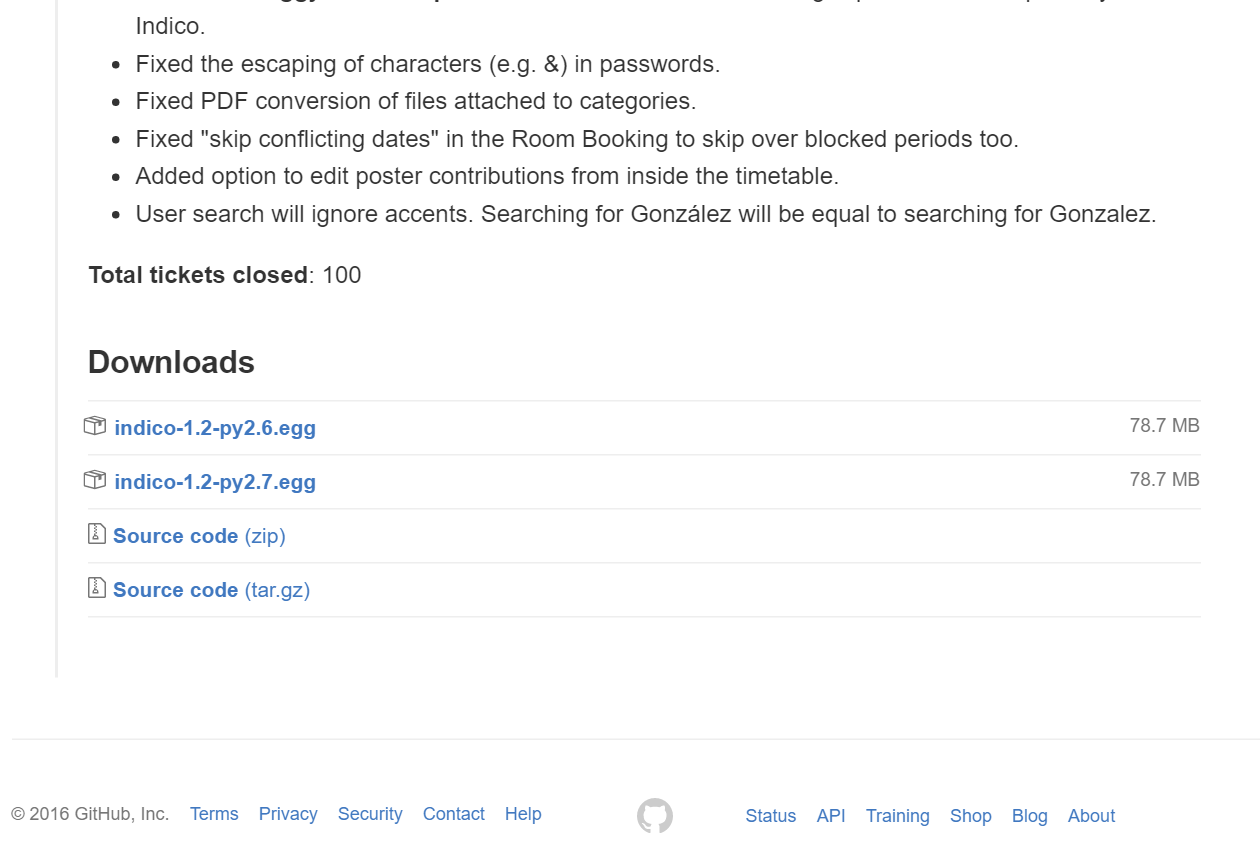
\includegraphics[scale=0.6]{1_2_assets.png}
        		\end{center}
        		\caption[Asset della release 1.2]{Asset caricati automaticamente per la release 1.2 di Indico su GitHub.}
        		\label{fig:1_2_asset}
        	\end{figure}
        
        \subsection{Upload su un server} \label{subsec:dp;ud;upload_server}
        
            L'upload a server è stato incluso come mezzo di diffusione alternativo di una distribuzione. Esso risulta molto più semplice rispetto all'upload su GitHub in quanto richiede soltanto di specificare l'indirizzo e la porta di accesso del server e i dati di autenticazione (username e chiave \ac{SSH}). Lo script si limiterà quindi ad invocare il comando \python{put()} di Fabric per copiare le distribuzioni generate nel percorso specificato sul server remoto.
            
            Le configurazioni per l'upload a server devono seguire la seguente struttura all'interno di \bash{fabfile.conf}:
            
            \begin{center}
                \begin{lstlisting}[language=python, gobble=18]
                    ssh = {
                        'host': 'remote-server.example.com',
                        'port': '22',
                        'user': 'root',
                        'key': '~/.ssh/id_rsa',
                        'dest_dir': '/path/on/remote/server'
                    }
                \end{lstlisting}
                \captionsetup{textformat=empty,labelformat=empty} \vspace{-2em}
                \captionof{lstlisting}[Configurazione per l'upload su server (esempio)]{Esempio di parametri di configurazione per l'upload su uno specifico server.}
            \end{center}
